\documentclass[a4paper,10pt,twocolumn]{article}
\usepackage[T1]{fontenc}
\usepackage[utf8]{inputenc}
\usepackage[italian]{babel}
\usepackage[top=3cm, bottom=3cm, left=2.5cm, right=2.5cm]{geometry}
\usepackage{graphicx}
\graphicspath{ ./images/} 


\begin{document}

\title{SIR Simulation}
\author{Lorenzo Manini \and Nicolò Montalti}
\date{A.A. 2019/2020}

\maketitle

\section{Descrizione del progetto}
\section{Compilazione ed esecuzione}

%ambiente per codice
\begin{verbatim}
    cmake ..
    make
\end{verbatim}

\section{Risultati}
Di seguito vengono riportati alcuni esiti di simulazioni effettuate variando i parametri delle classi \emph{Infection} e \emph{Motion}

\begin{figure}
    \caption{Simple Infection con infection probability = 0.05}
    \label{fig:simple_005}
    \centering
    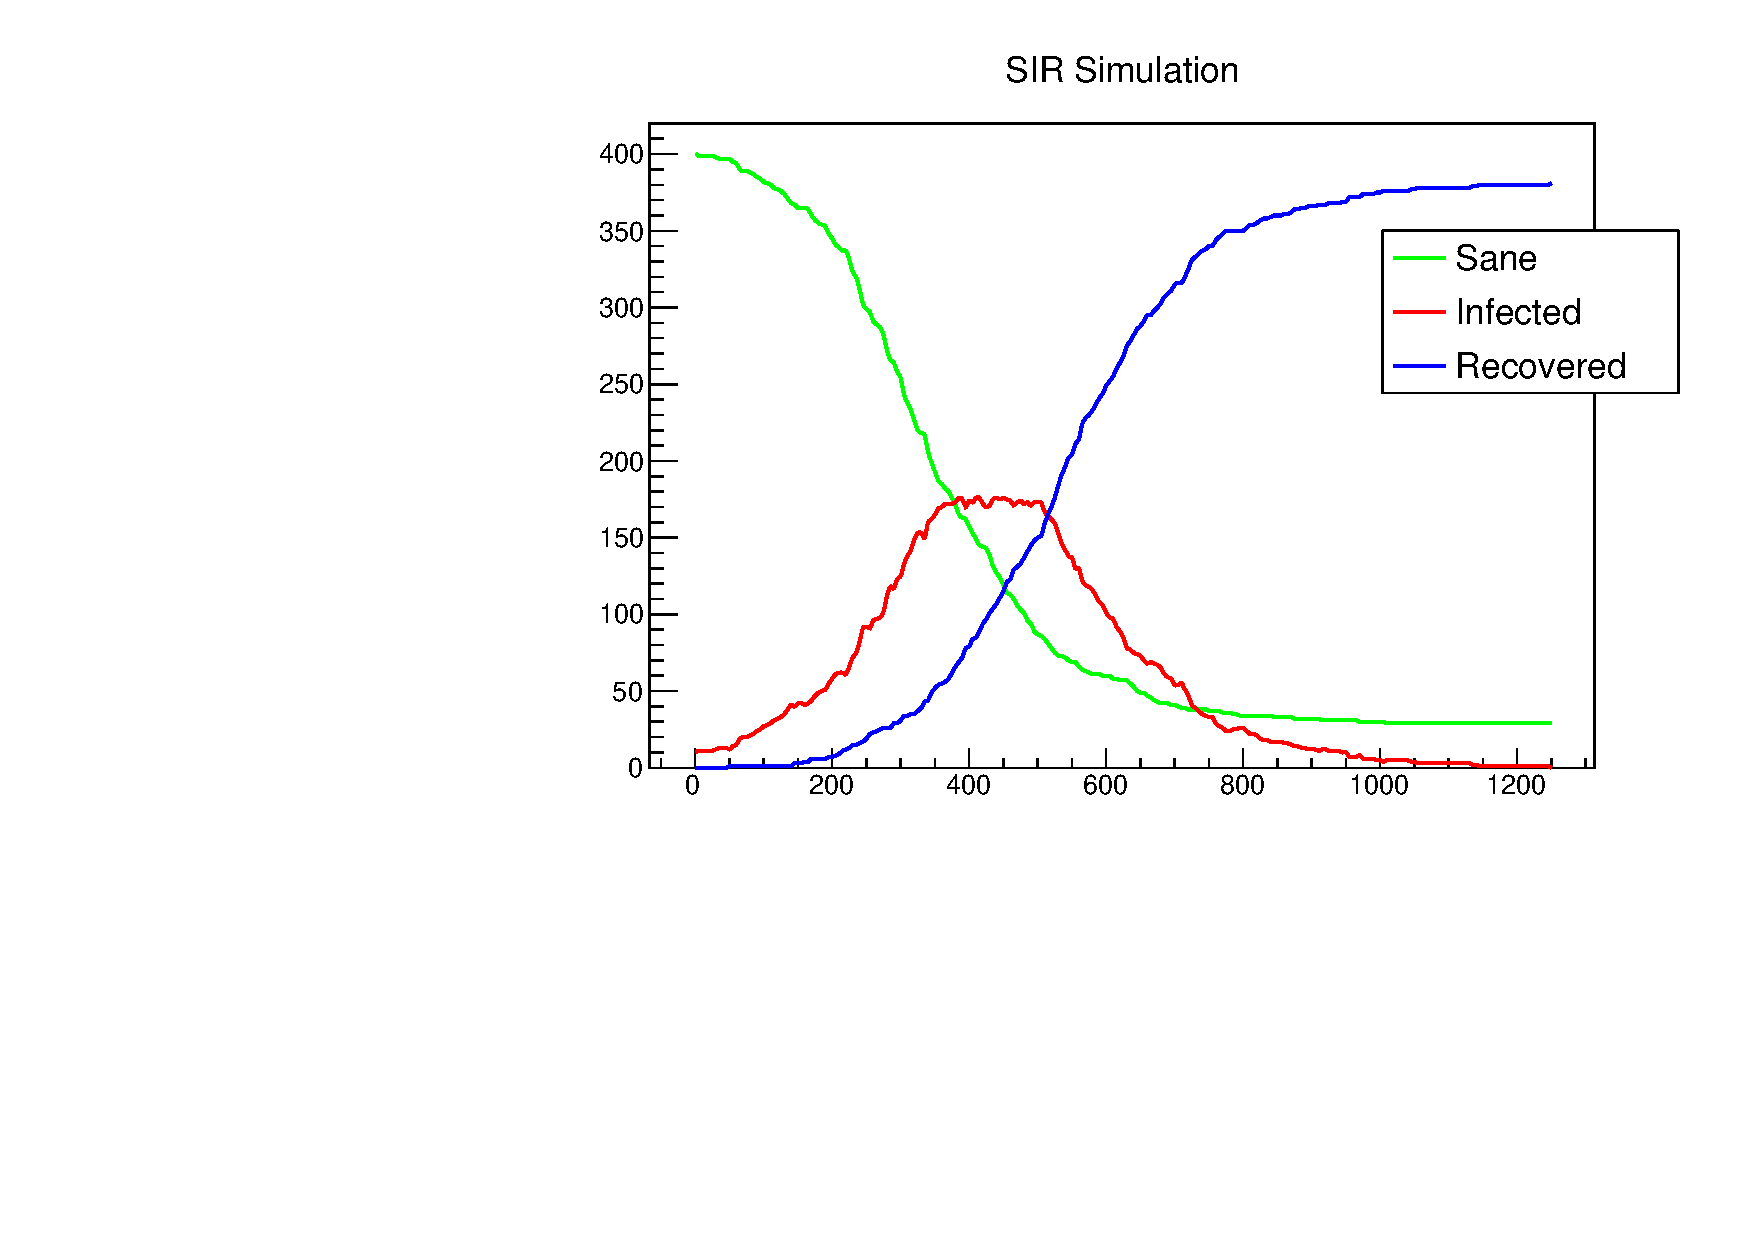
\includegraphics[width=\linewidth]{images/simple_0.05.pdf}
\end{figure}

\section{Strategie di testing}

\end{document}